\documentclass{article}
\usepackage{style}
\usepackage[utf8]{inputenc}
\usepackage{placeins}
\usepackage{booktabs} 
\usepackage{longtable}
\usepackage[title]{appendix}
\usepackage{amssymb}

\graphicspath{{media/}}

\title[Primality Testing]{Probabilistic Primality Testing and Analysis of Probabilistic AKS}
\author[Emilie Ma]{%
Emilie Ma\\%
University of British Columbia\\%
\texttt{kewbish@gmail.com}%
}
\date{\today}
\mentor{Pressiana Marinova\\%
Occado Technology Sofia\\%
\texttt{pressiana.marinova@gmail.com}%
}

\begin{document}
\maketitle
\newpage
\begin{abstract}
This paper aims to analyze the Fermat, the Euler (Solovay-Strassen), and the Miller-Rabin primality tests, three well-known probabilistic algorithms based on Fermat's little theorem. The Agarwal-Kayal-Saxena test, the first polynomial time deterministic primality test developed, is also discussed, as well as a proposal for a new probabilistic adaptation.
\end{abstract}

\section{Introduction}
Prime numbers, or numbers with no factors other than 1 and itself, are of crucial importance in cryptography and cybersecurity. Many encryption algorithms, such as the frequently used Rivest-Shamir-Adleman (RSA) cryptosystem, rely on the 'trapdoor' nature of prime numbers: while multiplying prime numbers is trivial, finding the factors of a composite number is computationally expensive. Since cryptography is so widely applied in modern systems, generating prime numbers for use in encryption cryptosystems is a major interest point and field of research in computer science and mathematics.

There is no known pattern to identify prime numbers, so to generate a prime number, a random number $n$ is first generated. This number $n$ is then passed through a primality test, or an algorithm designed to identify if a number is prime or not. A variety of algorithms may be used, including the Fermat, Euler or Solovay-Strassen, Miller-Rabin, and Agarwal-Kayal-Saxena (AKS) tests.

These tests, except the AKS test, are \emph{probabilistic}. A probabilistic test is an algorithm that utilizes some form of randomness in its design; for example, random trial bases may be selected from a range of possibilities. In contrast, a deterministic algorithm, when given an input, will always return the same output. Minimizing the running time of primality tests is desired to increase the efficiency of generating random primes, so often, probabilistic tests are used due to their shorter running time and increased practicality. However, probabilistic tests have a small probability of designating a number as prime when it is composite. This is avoided with deterministic primality tests, such as the AKS test discussed in section \ref{theory:aks}, but issues with impractical running times arise.

The AKS test is notable for being the first polynomial time deterministic primality test. Polynomial time refers to a concept of Big-O theory, or the notation that describes the upper bound of a function when its input tends towards infinity. In Big-O notation, polynomial time, or a function of form $O(n^x)$ is preferred to a function of form $O(x^n)$ for some input size $n$ and value $x$, as $x^n$ will grow faster than $n^x$ as $n$ increases. In other words, $n^x$ algorithms remain more efficient than $x^n$ ones in worst-case scenarios. 

However, even though AKS is bounded by a polynomial time, it remains impractical and incredibly slow compared to other probabilistic tests. As Richard Brent showed in a 2010 comparison with the Miller-Rabin and other probabilistic primality tests found that where 100 trials of Miller-Rabin took 0.3 seconds to process, AKS would take an estimated 37 weeks to run one trial on the same number (equivalent, as AKS is deterministic and only requires one run to determine the output). These times are unfeasible for applied usage, so research into optimizing and discovering probabilistic tests remains relevant.
% TODO: https://maths-people.anu.edu.au/~brent/pd/comp4600_primality.pdf
% TODO: https://ieeexplore.ieee.org/document/7942510
% TODO: http://depts.washington.edu/uwmxl/wordpress/wp-content/uploads/2017/05/AKS_Final_Report.pdf

As an alternative, this paper proposes a probabilistic version of AKS, inspired by methods used by the Fermat, Euler (Solovay-Strassen), and Miller-Rabin tests in choosing a range of random numbers to test against certain congruences and theorems.

\section{Background Number Theory}

Many probabilistic primality tests rely on number theory and modular arithmetic to test for primality. The Fermat, Euler (Solovay-Strassen), Miller-Rabin, and AKS tests and their background theory are discussed below.

Note that all $\log{n}$ in this paper are assumed to be taken as $\log_{2}{n}$ unless otherwise marked.

\subsection{Fermat Primality Test}
The Fermat Primality Test is a probabilistic primality test based on Fermat's little theorem.
Fermat's little theorem, developed by Pierre de Fermat in 1640, states that for any integer $a$ and any prime $p$, the following holds:
\[
    a^p \equiv a \pmod{p} 
\]
If $a$ is not divisible by, or \emph{coprime} to, p, the following is equivalent:
\[
    a^{(p - 1)} \equiv 1 \pmod{p} 
\]

\begin{proof} % https://artofproblemsolving.com/wiki/index.php/Fermat%27s_Little_Theorem
Consider $S = \{a, 2a, 3a, \ldots{}, (p - 1) * a\}$.
Suppose $ra$ and $sa$ in the set are equal $\pmod{p}$, so $r \equiv s \pmod{p}$.
Therefore, the $p - 1$ multiples of $a$ in $S$ are uniquely distinct, and must be congruent to ${1, 2, 3, \ldots{}, (p - 1)}$ in some order.
Multiply these congruences like so:
    \[a * 2a * 3a * \ldots{} * (p - 1)a \equiv 1 * 2 * 3 * \ldots{} (p - 1) \pmod{p}\]
This gives:
    \[a^{(p - 1)} * (p - 1)! \equiv (p - 1)! \pmod{p}\]
Divide by $(p - 1)!$ on each side for:
    \[a^{(p - 1)} \equiv 1 \pmod{p}\]
To arrive at the alternate form of Fermat's Little Theorem, multiply both sides by $a$.
    \[a^p \equiv a \pmod{p}\]
\end{proof}

Knowing that $a^{(n - 1)} \equiv 1 \pmod{n}$ holds if $n$ is prime, Fermat's primality test chooses $k$ random integers $a$ coprime to $n$ to test if all $a$ are congruent to 1. Because this holds trivially for $a \equiv 1 \pmod{n}$ and if $n$ is odd and $a \equiv -1 \pmod{n}$, $a$ is conventionally chosen such that $1 < a < n - 1$. Higher values of $k$ indicate a higher probability that the number is prime.

If $n$ passes these $k$ base tests, it is known as a probable prime. However, not all numbers that pass the Fermat primality test are prime - composite numbers $n$ that pass the test are known as Fermat pseudoprimes. There are infinitely many Fermat pseudoprimes, and several forms of composite numbers that pass the test. For example, Carmichael numbers, composite numbers that satisfy the relation $b^{(n-1)} \equiv 1 \pmod{n}$ for all integers $b$ coprime to $n$, all pass Fermat's primality test.

\subsection{Euler (Solovay-Strassen) Test} % https://artofproblemsolving.com/wiki/index.php/Euler%27s_Totient_Theorem
The Solovay-Strassen Test is another probabilistic test, utilizing the properties of Euler's theorem. Proposed by Leonhard Euler in 1763, Euler's theorem is a generalization of Fermat's little theorem, stating that if $a$ and $p$ are coprime, then the following holds:
\[
    a^{\phi(n)} \equiv 1 \pmod{n}
\]
The function $\phi(n)$ is Euler's totient function. The totient of some number $n$ is the number of positive integers $l$ in the range $1 \leq l \leq n$ where l is coprime to n.

\begin{proof}
    Consider $S = \{1 \leq l \leq n | gcd(l, n) = 1\} = \{l_1, l_2, l_3, \ldots{}, l_{\phi(n)}\}$.
    Create a set $aS = \{al_1, al_2, al_3, \ldots{}, al_{\phi(n)}\}$. \\
    All elements of $aS$ are relatively prime to $n$, so if all elements of $aS$ are distinct, $aS = S$. All elements of $aS$ are distinct, as all elements of $S$ are distinct. Therefore, each element of $aS \equiv S \pmod{n}$.
    Therefore:
    \[
        l_1 * l_2 * l_3 * \ldots{} * l_{\phi(n)} \equiv al_1 * al_2 * al_3 * \ldots{} * al_{\phi(n)} \pmod{n}
    \]
    As $l_1 * l_2 * l_3 * \ldots{} * l_{\phi(n)}$ is relatively prime to $n$, reducing this gives:
    \[
        a^{\phi(n)} * l_1 * l_2 * l_3 * \ldots{} * l_{\phi(n)} \equiv l_1 * l_2 * l_3 * \ldots{} * l_{\phi(n)} \pmod{n}
    \]
    Therefore, $a^{\phi(n)} \equiv 1 \pmod{n}$.
\end{proof}

Fermat's little theorem is considered a special case of Euler's theorem, because if $n$ is prime, $\phi(n) = n - 1$.

Given that $a^{\phi(n)} \equiv 1 \pmod{n}$, then 
\[
    a^{\phi(n) / 2} \equiv \begin{cases}
\;\;\,1\pmod{n}& \text{ when there exists }x \text{ such that }a\equiv x^2 \pmod{n}\\
     -1\pmod{n}& \text{ when there is no such integer.}
\end{cases}
\]

The conditions above form the criteria for the Legendre symbol of $a$ and $n$. The Legendre symbol $(\frac{a}{n})$ is defined like so:
\[
    (\frac{a}{n}) \begin{cases}
        0 & \text{ when $a \equiv 0 \pmod{n}$} \\
        -1& \text{ when $a \not\equiv 0 \pmod{n}$ and there exists $x: a \equiv x^2 \pmod{n}$} \\
     -1& \text{ when $a \not\equiv 0 \pmod{n}$ and there is no such integer $x$.}
\end{cases}
\]

The Jacobi symbol is the generalization of the Legendre symbol to any odd integer $n$, and is used in the Solovay-Strassen primality test. It is defined as the product of the Legendre symbols of $n$'s prime factors, such that:
\[
    (\frac{a}{n}) = (\frac{a}{p_1})^{\alpha_{1}} * (\frac{a}{p_2})^{\alpha_{2}} * \ldots{} * (\frac{a}{p_k})^{\alpha_{k}}
\]
for $n = p_1^{\alpha_{1}} * p_2^{\alpha_{2}} * \ldots{} * p_k^{\alpha_{k}}$.

As with Fermat's primality test, $k$ random bases $a$ are tested. If $a^{(n - 1) / 2} \equiv (\frac{a}{n}) \pmod{n}$ holds for all $k$ basis, then $n$ is a probable prime.

Similar to Fermat's primality test, the Solovay-Strassen test may pass composite numbers as primes. These are then known as Euler (sometimes Euler-Jacobi) pseudoprimes or liars. All Euler pseudoprimes are also Fermat pseudoprimes. 

\subsection{Miller-Rabin Primality Test} % http://home.sandiego.edu/~dhoffoss/teaching/cryptography/10-Rabin-Miller.pdf
A third probabilistic primality test, the Miller-Rabin primality test was developed first by Gary Miller in 1976, and subsequently modified by Michael Rabin in 1980. The test relies on two congruence relations that hold when $n$ is an odd prime and rewritten as $2^s * d + 1$, and $a$ is a base such that $0 < a < n$:
\begin{gather*}
    a^d \equiv 1 \pmod{n} \\
    a^{(2^r * d)} \equiv -1 \text{ for some $r$ such that $0 \leq r < s$}
\end{gather*}

Because $n$ is written as $2^s * d + 1$, $n - 1 = 2^s * d$. Therefore, if $a^d \equiv \pm 1 \pmod{n}$, then $n$ is a strong probable prime.

\begin{proof}
    Given that:
    \[
        a^{(n - 1)} \equiv (a^d)^{2^s} \equiv 1 \pmod{n}
    \]
    for all prime $n$, and because there are no square roots of 1 other than $\pm 1$, the repeated squaring with $2^s$ doesn't affect the congruence.
\end{proof}

Otherwise, $a^d \pmod{n}$ is squared, for $a^2d$. If $a^2d \equiv 1 \pmod{n}$, n is composite, because there are different square roots of $a^2m \pmod{n}$ other than $\pm 1$. If $a^2d \equiv -1 \pmod{n}$, then $n$ is a probable prime for similar reasons as above.

These checks are repeated until $a^{(2^{(s - 1)} * d)}$ has been reached. If it is $\pm 1$, the result is known by the tests above; however, if not, $n$ is composite, by Fermat's little theorem.

\subsection{Agarwal-Kayal-Saxena (AKS) Primality Test} % https://www.cse.iitk.ac.in/users/manindra/algebra/primality_v6.pdf
\label{theory:aks}
By contrast, the AKS primality test is a deterministic primality test first proprosed by Manindra Agarwal, Neeraj Kayal, and Nitin Saxena in 2002. It is the first primality test to deterministically verify primality in polynomial time for all number inputs, with a time complexity bound of $\mathcal{O}(\log{(n)}^{15/2})$.

The test is based on the theorem that an integer $n >= 2$ and an integer $a$ coprime to $n$, $n$ is prime if and only if the below holds within the polynomial ring $\mathbb{Z}[x]$, or the ring of polynomials with degree at most $n$ over $\mathbb{Z}$.
\[
    (X + a)^n \equiv X^n + a \pmod{n}
\]

\begin{proof} % http://www.cs.tau.ac.il/~amnon/Classes/2019-Derandomization/Lectures/Lecture7-AKS-All.pdf
    This is a generalization of Fermat's little theorem over polynomials, proven with the binomial identity.
    \[
        (x + a)^n = \sum_{i=0}^{n} \binom{n}{i} x^i a^{n - i} where \binom{n}{0} = \binom{n}{n} = 1
    \]
    If $n$ is prime, then:
    \[
        \binom{n}{i} = \frac{n (n - 1) \ldots{} {n - i + 1}}{i!}
    \]
    for all i > 1. When taken $\pmod{n}$, $n$ divides the numerator once; therefore, $\binom{n}{i} \equiv 0 \pmod{n}$. $a$ does not necessarily need to be coprime with $n$.
    If $n$ is not prime, and $a$ is coprime with $n$, then $n$ has a prime factor of form $p^k$. $p^k$ will divide $n$, but $p^{k - 1}$ will not. Given the monomial with a coefficient of:
    \[
        \binom{n}{i} = \frac{n (n - 1) \ldots{} {n - p + 1}}{p!}
    \]
    $p^k$ divides $n$, but not $(n - 1) \ldots{} (n - p + 1)$. Therefore, $p^k \vert n (n - 1) \ldots{} (n - p + 1)$ but $p^{k + 1} \nmid n (n - 1) \ldots{} (n - p + 1)$. $p$ also divdes $p$, but not $1 \ldots p$, so $p \vert p!$ but $p^2 \nmid p!$. This gives $p^{k - 1} \vert \binom{n}{p}$ and $p^k \nmid \binom{n}{p}$. As $p^k$ is a factor of $n$, $n \nmid \binom{n}{p}$, and $x^p$ does not vanish.
\end{proof}

The steps of the algorithm are as follows:
\begin{enumerate}
    \item The test begins by ensuring $n$ is not a perfect power, or a number of form $a^k$ for some $a$ and $k$. If it is, the number is composite.
    \item Next, the algorithm finds the smallest $r$ such that $ord_r(n) > {\log{n}}^2$ and $r$ is coprime to $n$.
    \item The algorithm then checks for all $2 \leq a \leq min(r, n - 1)$ that $a \nmid n$. If $a \vert n$ for some $a$ in this range, the number is composite. This is equivalent to trial division up to $r$.
    \item If $n \leq r$, the number is prime, as this is equivalent to trial division to $\sqrt{n}$.
    \item The last step of the algorithm reduces the time complexity from exponential to polynomial time by operating over the finite ring $(\mathbb{Z}/(n))[X] / (X^r - 1)$. Each $a$ from $1 \leq a \leq \lfloor \sqrt{\varphi(r)}\log(n) \rfloor$ is checked for the generalized Fermat's theorem. If it does not pass, the number if composite; if it passes, the number is prime.
\end{enumerate}

\section{Running Time}
This section discusses the running time bounds of the tests with Big-O notation.

In Big-O notation, $\widetilde{O}(f(n))$ is a shorthand for $O(f(n) * log{f(n)}^k)$ for some $k$, ignoring the logarithm factor due to the growth effects of other operations in $f(n)$.

\subsection{Fermat Primality Test}
The Fermat primality test implementation tested used repeated squaring and multiplication techniques, requiring several modular computations per bit of each number $n$ tested. The number of bits in $n$ is $\log{n}$, so as there are $k$ iterations of a modular exponentiation applied, the final complexity is $O(k * log{n})$.

\subsection{Euler (Solovay-Strassen) Primality Test}
The Euler (Solovay-Strassen) primality test is implemented in three main steps: the coprime to $n$ check, the computation of the Jacobi symbol $(\frac{a}{n})$, and the modular exponentiation.Checking if a number is coprime to another involves a greatest-common-denominator test, which can be run in a time of $O(log{n})$ where $log{n}$ is again the size of the number in bits. Similarly, the Jacobi symbol and modular exponential can both also be run in $O(log{n})$ time, so the final complexity is:
\[
    O(k * log{n} * log{n} * log{n}) = O(k * log^3{n})
\]

\subsection{Miller-Rabin Primality Test}
Similar to the Euler (Solovay-Strassen) test, the Miller-Rabin test runs in $O(k * log^3{n})$ time, due again to the modular exponentiation operations.

\subsection{AKS Primality Test}
The AKS paper originally detailed the time complexity of the algorithm as $\widetilde{O}(log(n)^{12})$ with the use of fast modular exponentiation techniques (like repeated squaring). However, the paper was later revised to give the time complexity $\widetilde{O}(log(n)^{15/2})$ based on new theory and proofs.

In 2005, after Pomerance and Lenstra developed an AKS variant with a running time of $\widetilde{O}(log(n)^{6})$, the paper was again updated.

\section{Probabilistic AKS}

As noted before, the AKS primality test is deterministic: with any given input, the algorithm will consistently return the same output. None of the AKS algorithms, including additional improvement proposals, include any element of randomization. However, inspired by the choice of random bases in the Fermat, Euler, and Miller-Rabin tests, this paper proposes a probabilistic version of the AKS algorithm. (To prevent confusion, the original AKS test as proposed by Agarwal, Kayal, and Saxena will henceforth be referred to as deterministic AKS, while the new proposed algorithm will be referred to as probabilistic AKS.) This probabilistic AKS test relies on much of the same background theory of polynomial equivalences as the deterministic AKS test. The modifications to the original AKS test are as follows:

\begin{itemize}
    \item Compute steps 1 through 4 following the deterministic AKS algorithm.
    \item Take a parameter $k$, such that $1 \leq k \leq \lfloor \sqrt{\varphi(r)}\log(n) \rfloor$.
    \item Instead of verifying that $(X + a)^n \equiv X^n + a \pmod{X^r - 1, n}$ for all $1 < a < \lfloor \sqrt{\varphi(r)}\log(n) \rfloor$, check only for $k$ random $a$ values in that range.
    \item If $n$ passes these tests, $n$ is prime; otherwise, it is composite.
\end{itemize}

\subsection{Running Time}
This probabilistic AKS variant was derived from an implementation of the improved deterministic AKS test proposed in 2004 by Agarwal, Kayal, and Saxena. As such, the theoretical running bound for the original implementation without modifications is $\widetilde{O}(log(n)^{15/2})$.

However, as this probabilistic variant reduces the number of polynomial equalities checked from a maximum of $\lfloor \sqrt{\varphi(r)}\log(n) \rfloor$ to $k$, a factor of $log(n)$ can be removed, and replaced with a $k$. The final bound of probabilistic AKS is proposed to be $\widetilde{O}(k * log(n)^{13/2})$. However, this has not yet been theoretically verified, and only empirically shown.

\subsection{Effects on Pseudoprimes}
By introducing a factor of randomization into the deterministic AKS algorithm, the probabilistic AKS algorithm therefore has some probability that a composite number will be passed as prime, since not all the polynomial equalities are verified. These will be referred to as probabilistic AKS pseudoprimes.

\emph{Hypothesis.} Like other probabilistic primality tests, the likelihood of passing a pseudoprime is expected to decrease with increased $k$ values such that more polynomial equivalences are verified. The amount of pseudoprimes passed with reasonably high $k$ values, an arbitrary value proposed to be perhaps $10 * \log{n}$ to represent a reasonable percentage of all possible polynomial equivalences, is expected to be between the number of Miller-Rabin pseudoprimes identified and passed, and the number of pseudoprimes passed by deterministic AKS, namely zero.

\section{Methods}
The primality tests were subject to a similar analysis method over multiple trials; the raw data is available in Appendix \ref{appendix:data}. For the probabilistic tests, each trial tested a different $k$ value, and consisted of:

\begin{itemize}
    \item{Generating a random set ($S$) of $10^4$ odd integers such that $10^5 < x < 10^6$. This interval was chosen due to an intersection of higher concentrations of pseudoprimes found for meaningful data comparisons between each trial and reasonable running times for the trials conducted.}
    \item{Using Sympy's \texttt{is\_prime} (which runs a variant of the Baillie-Pomerance-Selfridge-Wagstaff probabilistic primality test) to check for primality for each integer in $S$}
    \item{Running the primality test with $k$ attempts run on each integer in $S$ with respect to some base $a$}
    \item{Counting all pseudoprimes which passed the primality test but not Sympy's primality test}
    \item{Return lowest number of bases tried (lowest $k$) that returned the lowest number of pseudoprimes passed, the maximum and minimum number of pseudoprimes, and the average pseudoprimes found}
\end{itemize}

Each trial was timed with the Python \texttt{timeit} command, recording the total wall time elapsed. Data for average time taken per $k$ value was collected in a similar way. 

For the Fermat, Euler (Solovay-Strassen), and Miller-Rabin tests, the results of fifty trials were recorded, ranging from $k = 1$ to $k = 100$.

Deterministic AKS has been proven, so data was not recorded with respect to base analysis. A trial of the first $10^4$ integers took around 118 min, and fifty trials would have been impractical for the scope of this inquiry. The data included in Appendix \ref{appendix:data} includes recorded times elapsed for timing ten trials of fifty random integers in the range $10^5 \leq x \leq 10^6$. % TODO

For probabilistic AKS, the testing method consisted of running ten trials over a random set $S$ with $10^2$ elements tested and the same range as the Fermat, Euler, and Miller-Rabin tests. However, only $k$ values of $1 \leq k \leq 10$, 100, 200, 300, and 400 were tested. The upper bound $\lfloor \sqrt{\varphi(r)}\log(n) \rfloor$ was found to be around 400 for the range tested, so these $k$ values were selected to show the performance of the test at different $k$ intervals over the possible range. These smaller bounds for analysis were also used due to practical reasons, as a trial of the first $10^4$ integers with $k = 50$ took over 508 min. This elapsed time would increase with the larger numbers in the range used for testing, making gathering data impractical for the scope of this paper. Data is also recorded for the time required to run ten trials of fifty random integers, similar to the deterministic AKS data. % TODO

The raw data of each of the primality tests can be found in Appendix \ref{appendix:data}.
See Appendix \ref{appendix:tech} for primality test implementation details and hardware specifications.

\section{Results}
For the Fermat, Euler (Solovay-Strassen), and Miller-Rabin tests, the results of trials ranging from $k = 1$ to $k = 50$ are shown. For $k$ values greater than 50, it was found that pseudoprimes were found very rarely (around 5 pseudoprimes found in total over 50 trials of $50 \leq k \leq 100$) across all three tests. Additional base analysis data, including that for $k$ values greater than 50, can be found in Appendix \ref{appendix:data}. As 

In Figure \ref{fig:pprimes_v_bases}, the average number of pseudoprimes passed per $k$ bases tested is shown. All test exhibit a similar pattern of passing larger number of pseudoprimes with lower amounts of bases tested $k$. The Fermat primality test passed the most pseudoprimes, with an average of 6.5 pseudoprimes at $k = 1$. The Euler (Solovay-Strassen) test passed an average of 3.2 pseudoprimes at $k = 1$, while the Miller-Rabin test passed a similar average of 3.3. The Fermat primality test has low ($<0.1$) average numbers of pseudoprimes passed beginning around $k = 25$. The Euler test passes low numbers of pseudoprimes at around $k = 5$, and at $k = 3$, the Miller-Rabin test begins to pass low numbers of pseudoprimes. Both the Euler and Miller-Rabin tests pass consistent averages of 0 pseudoprimes after their respective drop-off points; however, the Fermat test wavers around 0 to 0.1 pseudoprimes passed for all trials after $k = 25$.

Figure \ref{fig:time_v_bases} shows the time elapsed for $k$ base trials over $k$ bases tested. Each of the tests shows an increase in time required to test a number as $k$ also increases. All three tests average around 3sec for $k = 1$, but this quickly drops and subsequently begins to increase again. The figure shows several spikes in time elapsed, but overall trends for each of the tests are clear. The Fermat primality test shows the steepest upwards trend, followed by the Miller-Rabin test, while the Euler (Solovay-Strassen) test exhibits a more consistent but slight downwards slope. The Fermat primality test has a slope of around 0.027sec per $k$ increase, while the Miller-Rabin test shows around 0.01sec per $k$ increase. The slope of the Euler test appears to be -0.01sec per $k$ increase, though the trend only continues until around $k=30$ before flattening out. The maximum time required for the Fermat test after the initial spike at $k=1$ was 4.290sec at $k=44$, and the minimum 1.929sec at $k=2$. The Miller-Rabin test had slightly lower maximums and minimums: 3.604sec at $k=27$ and 1.944sec at $k=4$. The Euler test had the lowest times, with a maximum of 2.279sec at $k=4$ and a low point of about 1.291s from $k=36$ to $k=50$.

Figures \ref{fig:pprimes_v_trial} and \ref{fig:time_v_trial} show the average pseudoprimes passed and running time elapsed over several cross-base trials (trials testing all $k$ values from 1 to 100, or 1 to 50). The Fermat Primality test has a higher average than the other two tests, averaging around 0.2327 pseudoprimes passed per $10^4$ random numbers tested. The Euler (Solovay-Strassen) and Miller-Rabin average similar values of 0.0380 and 0.0303 pseudoprimes passed, respectively. The Fermat primality test passed a maximum of 0.3838 average pseudoprimes, and a minimum of 0.0808 pseudoprimes. Unlike the Euler and Miller-Rabin tests, the Fermat test did not reach an average of 0.0000 pseudoprimes over any of its trials. The Euler test passed a lower range of numbers of pseudoprimes, with a maximum of 0.1010 and a minimum of 0.0000 pseudoprimes passed. The lowest range of pseudoprimes passed is shown by the Miller-Rabin test, which passed a maximum of 0.0808 and a minimum of 0.0000 pseudoprimes.

The trends in figure \ref{fig:time_v_trial} show a clear hierarchy of running time elapsed over the cross-base trials. Each of the tests has a stable running time, with the Fermat primality test running in an average of 8.339sec, the Miller-Rabin next with an average of 6.368sec, and the Euler (Solovay-Strassen) test with the lowest average of 4.073sec. The running time for the Fermat test ranged from 7.737 to 11.430 seconds, the highest of the primality tests. The Miller-Rabin test had a higher range than the Euler test as well, with a range of 5.849 to 8.569 seconds compared to the Euler test's range of 3.662 to 5.325 seconds.

\FloatBarrier
\begin{figure}[h!]
\caption{The effect of increasing the number of base trials $k$ on pseudoprimes passed}
\label{fig:pprimes_v_bases}
\centering
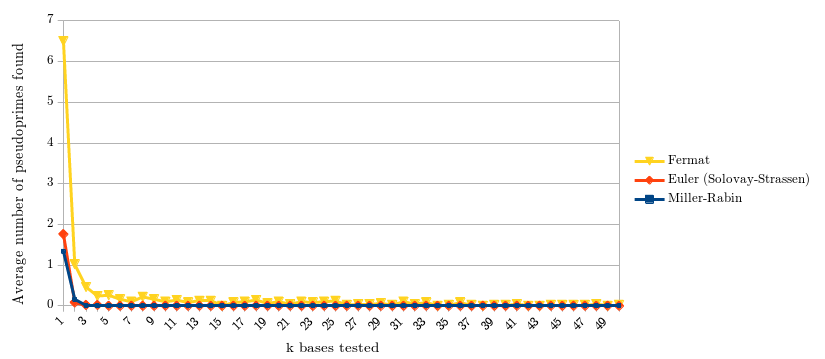
\includegraphics[width=\textwidth]{pprimes_v_bases}
\end{figure}
\FloatBarrier

\FloatBarrier
\begin{figure}[h!]
\caption{The effect of increasing the number of base trials $k$ on running time elapsed}
\label{fig:time_v_bases}
\centering
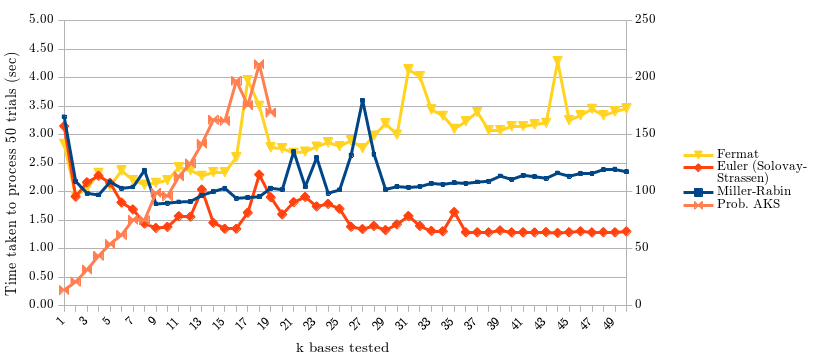
\includegraphics[width=\textwidth]{time_v_bases}
\end{figure}
\FloatBarrier

\FloatBarrier
\begin{figure}[h!]
\caption{Average pseudoprimes passed across all $1 \leq k \leq 50$ values per trial}
\label{fig:pprimes_v_trial}
\centering
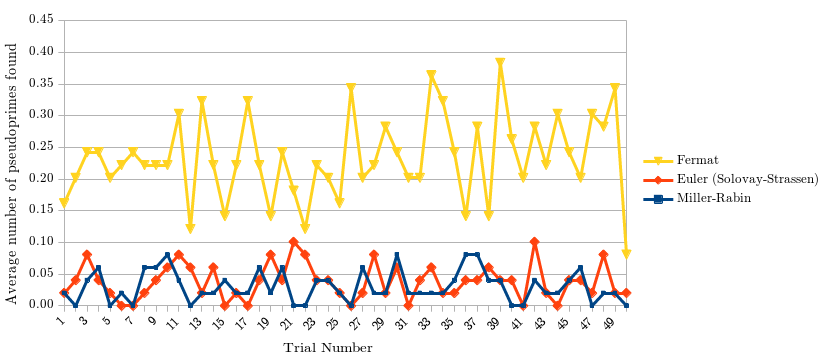
\includegraphics[width=\textwidth]{pprimes_v_trial}
\end{figure}
\FloatBarrier

\FloatBarrier
\begin{figure}[h!]
\caption{Running time elapsed across all $1 \leq k \leq 100$ values per trial}
\label{fig:time_v_trial}
\centering
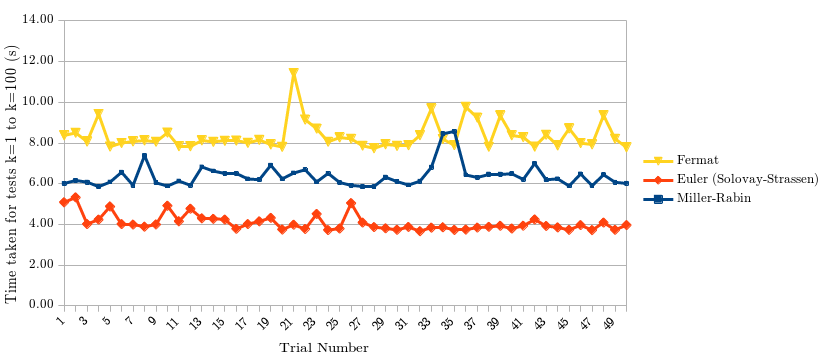
\includegraphics[width=\textwidth]{time_v_trial}
\end{figure}
\FloatBarrier

% TODO: det AKS vs prob AKS

\section{Discussion}
Discussion

\subsection{Sources of Error}
\label{soe}
A possible source of error present includes the range of numbers tested for pseudoprimes and the distribution of pseudoprimes over said range. % TODO: https://cr.yp.to/bib/1980/pomerance-pseudo.pdf
As Pomerance, Selfridge, and Wagstaff showed in their 1980 analysis on pseudoprimes to $25 * 10^9$, there are 167 Fermat pseudoprimes, 78 Euler (Solovay-Strassen) pseudoprimes, and 30 strong (Miller-Rabin) pseudoprimes between $10^5$ and $10^6$. These values increase for higher numbers, and it is possible that the bounds of $10^5 \leq n \leq 10^6$ chosen for all $n$ tested in each trial were insufficient to reveal unexpected behaviour of the primality tests analyzed that may occur with different bounds.

Another potential source of error was the $k$ value analysis for the probabilistic AKS test. Due to time constraints, only certain $k$ values were tested, with smaller numbers of random integers tested with each trial ($10^2$ instead of $10^4$). These $k$ values were not the same as the ones tested in the Fermat, Euler, and Miller-Rabin trials, which may not allow for standardized comparisons. The same number of trials was also not conducted (10 vs 50) due to time constraints, which may lead to outlier trials overly affecting the averages for the probabilistic AKS trials.

\subsection{Further Research}
As mentioned in section \ref{soe}, the distribution of pseudoprimes for each of the tests varies with the upper and lower bounds chosen. In larger intervals between larger numbers, the amount of these pseudoprimes grows. However, with larger intervals, the probability of randomly selecting pseudoprimes within $10^4$ choices decreases. Increasing the bounds of the tests was outside the scope of this examination, but may be left to future research. Running the primality tests over a larger interval of larger numbers with a higher amount of choices may improve this analysis. 

As well, the $k$ values in data collected for the probabilistic AKS test were not identical to those analyzed for the Fermat, Euler, and Miller-Rabin tests. With values of $1 \leq k \leq 50$, however, it was unlikely reasonable analysis could be done, as the number of equations tested was too low to give any meaningful results. In the future, finding the approximate range of $k$ where the number of pseudoprimes found begins to range similarly to the values found at $1 \leq k \leq 50$ for the other probabilistic tests may allow closer comparison between these primality tests. As well, running additional trials (50 total) for each of the $k$ values for the probabilistic AKS test will allow for a larger overview of the test's performance to be formed.

\section{Conclusion}
Conclusion + industry applications of this research

\nocite{*}
\bibliographystyle{plainnat}
\bibliography{references}

\appendix
\begin{appendices}
\section{Raw Data for Primality Tests} \label{appendix:data}

The raw data for each of the primality tests can be found \href{https://github.com/kewbish/srs/tree/master/scripts/dataset}{here}. % TODO: Ensure correct link if I restructure files
The data is available in CSV format, labelled by primality test (Fermat, Euler, Miller-Rabin, deterministic AKS, and probabilistic AKS). The folder also includes other data not discussed in-depth in this paper, including several base analysis types (all bases generated randomly, base 2, base 3, base 5, or a combination of bases 2 and 3, bases 3 and 5, and bases 2 and 3).

Each row in the CSV file is a trial of the given test with given base. The first hundred columns represent the pseudoprimes found at $k$ trials of different bases. The last four columns represent the average pseudoprimes found over the entire trial from $1 \leq k \leq 100$, the lowest $k$ value required to pass the lowest number of pseudoprimes, the lowest number of pseudoprimes, and the time required to run the test in minutes and seconds. 
The last row, which contains only 50 values, should be interpreted as the average time taken for a trial of $k$ bases, where $k$ is the column number.

\section{Technical Details} \label{appendix:tech}

\subsection{Primality Test Implementations}
The implementations of the primality tests can be found on GitHub at kewbish/srs. % TODO: citation on GitHub
The tests were implemented with Python 3.7, with the Numpy and Numba libraries used to optimize computations, and the Sympy library used to test for primality.
The AKS primality test implementation was iterated on from a reference implementation by Sophoclis Stephanou was found on GitHub. % TODO: citation

\subsection{Hardware}
The primality tests ran on a HP-15bs028ca running Manjaro Linux x86\_64 and kernel 5.10.49-1-MANJARO, with a 4-core Intel i5-7200U 3.100GHz CPU and 16.0GiB of RAM.

\end{appendices}

\end{document}

